\section{Testable Predictions}\label{sec:predictions}

\subsection{Double Slit Residual Fringes}
The total phase includes:
\begin{equation}
\Delta\phi = \Delta\phi_{\text{path}} + \Delta\phi_\theta.
\end{equation}
Figure~\ref{fig:double-slit-sweep} shows simulated fringe shifts for a drive-locked $\theta$ modulation.

\begin{figure}[h]
  \centering
  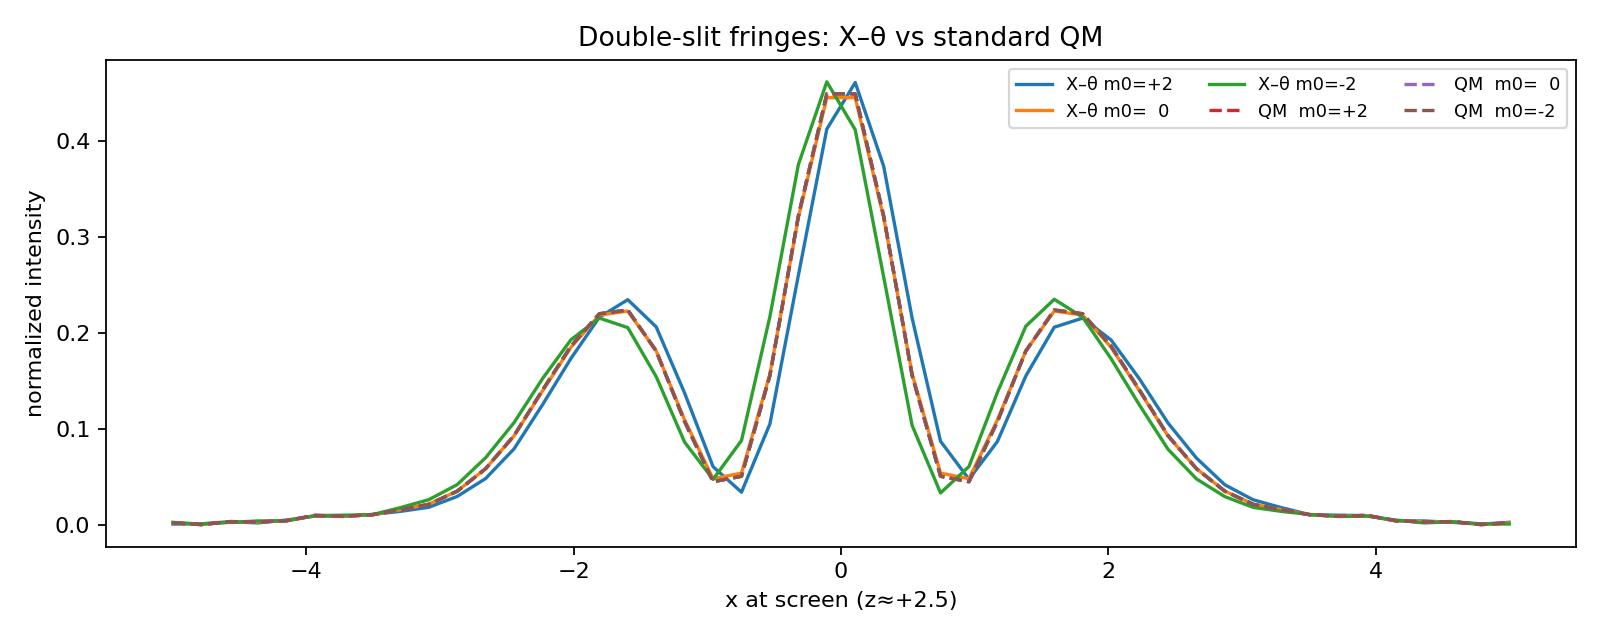
\includegraphics[width=0.85\linewidth]{double_slit_sweep.png}
  \caption{Predicted fringe shift vs $\theta$-drive amplitude and frequency (simulation).
  Null-EM conditions isolate $\Delta\phi_{\theta}$.}
  \label{fig:double-slit-sweep}
\end{figure}

\subsection{Photoelectric Effect Modifications}
Our framework predicts that $\theta$ introduces an internal quantized energy channel,
slightly shifting the classical cutoff frequency.

\begin{figure}[h]
  \centering
  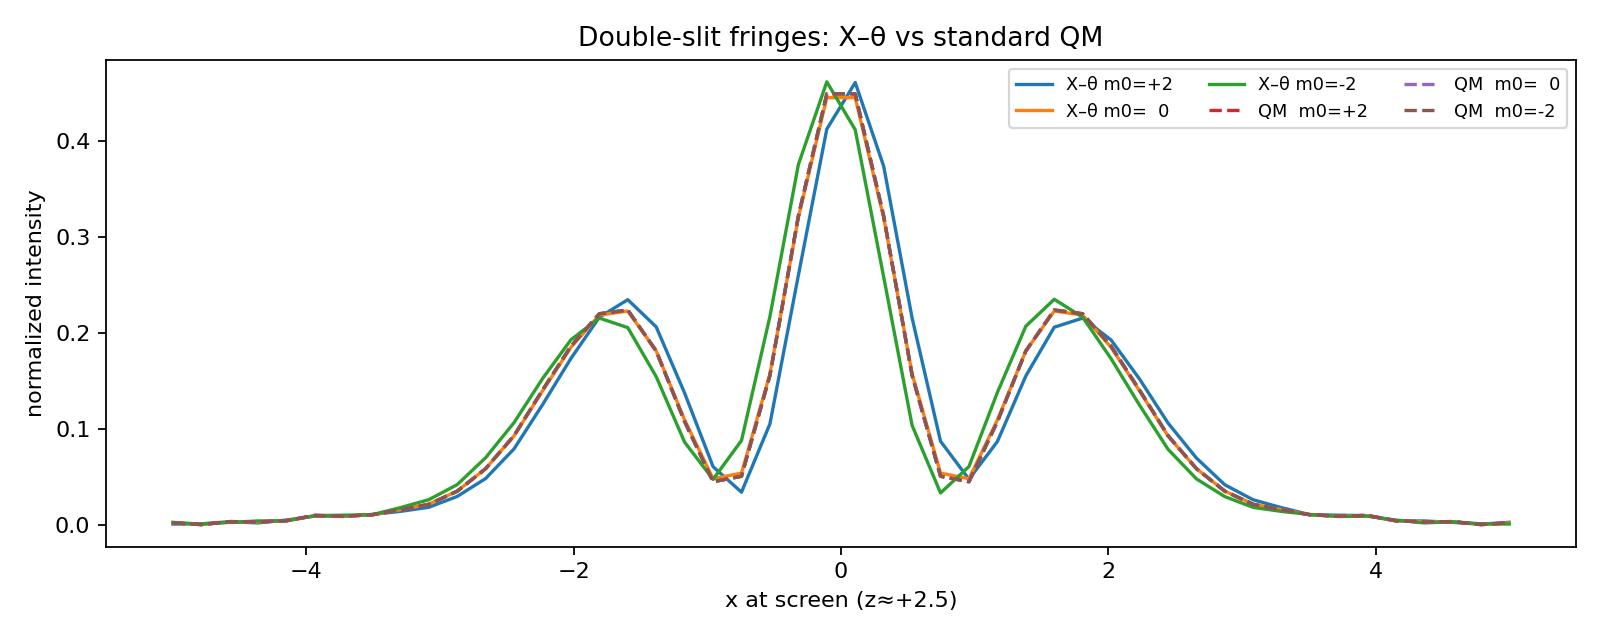
\includegraphics[width=0.85\linewidth]{photoelectric_theta.png}
  \caption{Simulated photoelectric threshold shifts due to $\theta$.
  Internal energy exchange modifies the cutoff frequency.}
  \label{fig:photoelectric-theta}
\end{figure}

\subsection{Black Hole Orbits and Singularities}
Adding $\theta$ modifies geodesics near compact objects, softening singularities.

\begin{figure}[h]
  \centering
  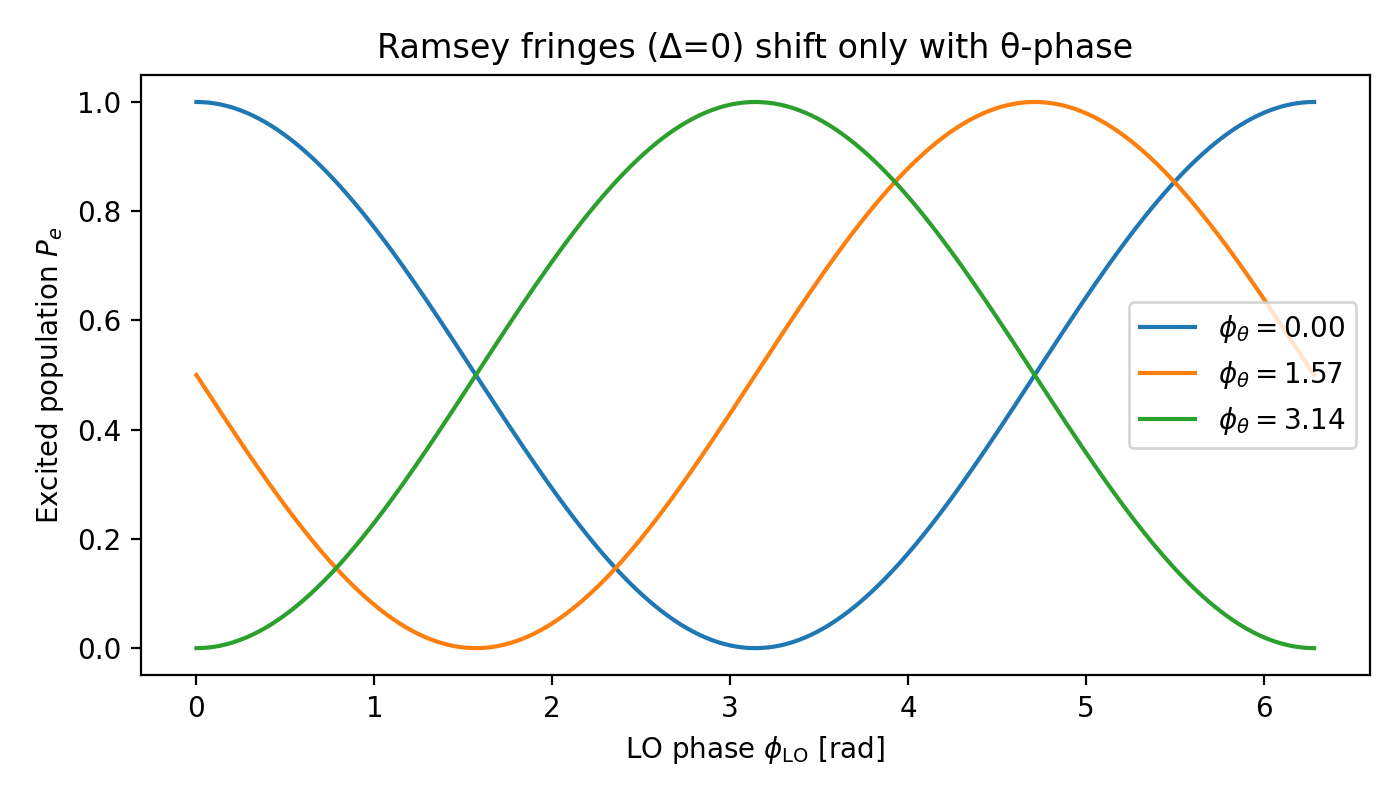
\includegraphics[width=0.85\linewidth]{blackhole_orbits_theta.png}
  \caption{Numerical orbits near a black hole with $\theta$ correction.
  The $\theta$-Lorentz term alters trajectories and reduces singularity strength.}
  \label{fig:blackhole-orbits}
\end{figure}

\subsection{Gravitational Wave Birefringence}
The X--$\theta$ framework predicts splitting of left- and right-handed gravitational wave polarizations.

\begin{figure}[h]
  \centering
  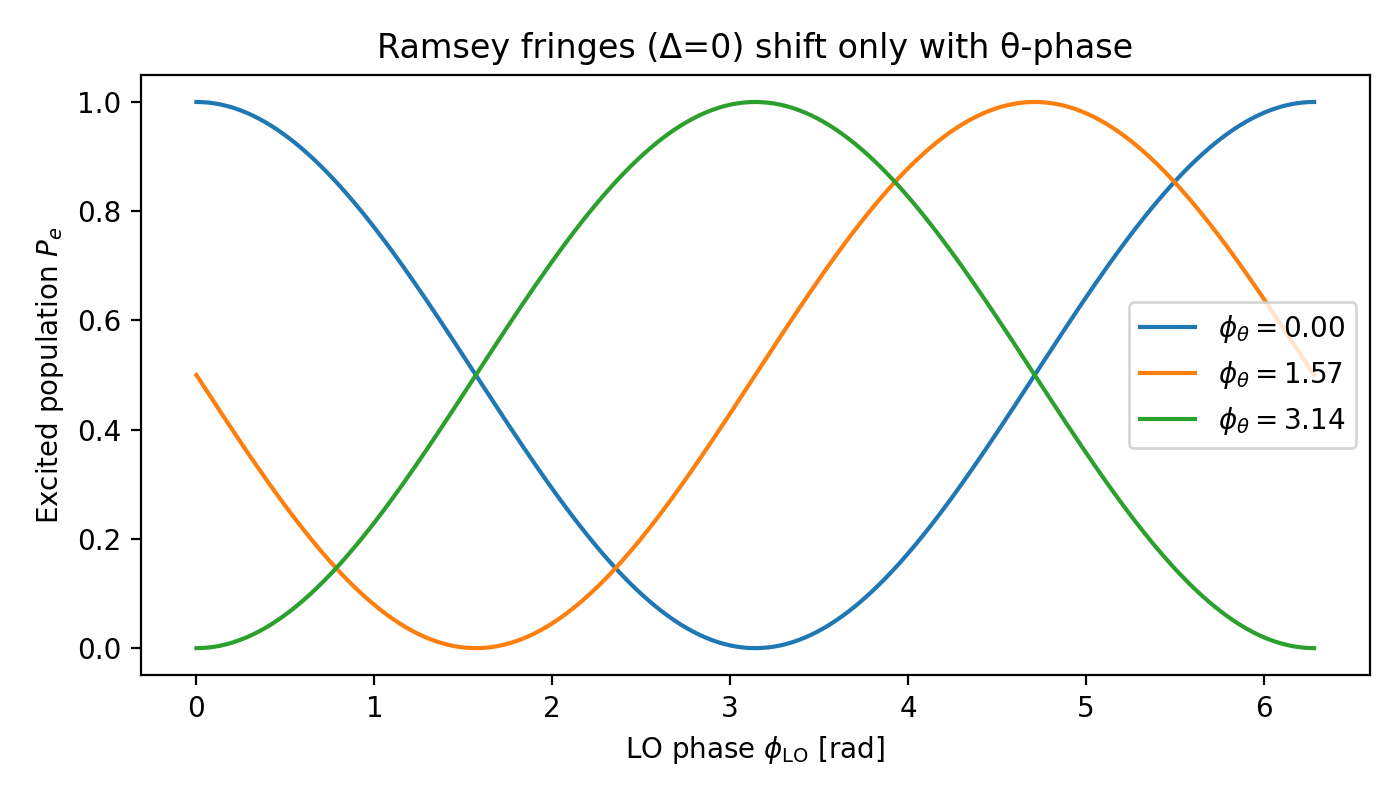
\includegraphics[width=0.85\linewidth]{gw_birefringence_theta.png}
  \caption{Predicted gravitational wave birefringence due to $\theta$.
  Polarization states acquire different effective propagation speeds.}
  \label{fig:gw-birefringence}
\end{figure}

\subsection{Neutron and Atom Interferometry}
Even under null electromagnetic conditions, $\theta$ introduces new phase shifts observable in interferometry.

\begin{figure}[h]
  \centering
  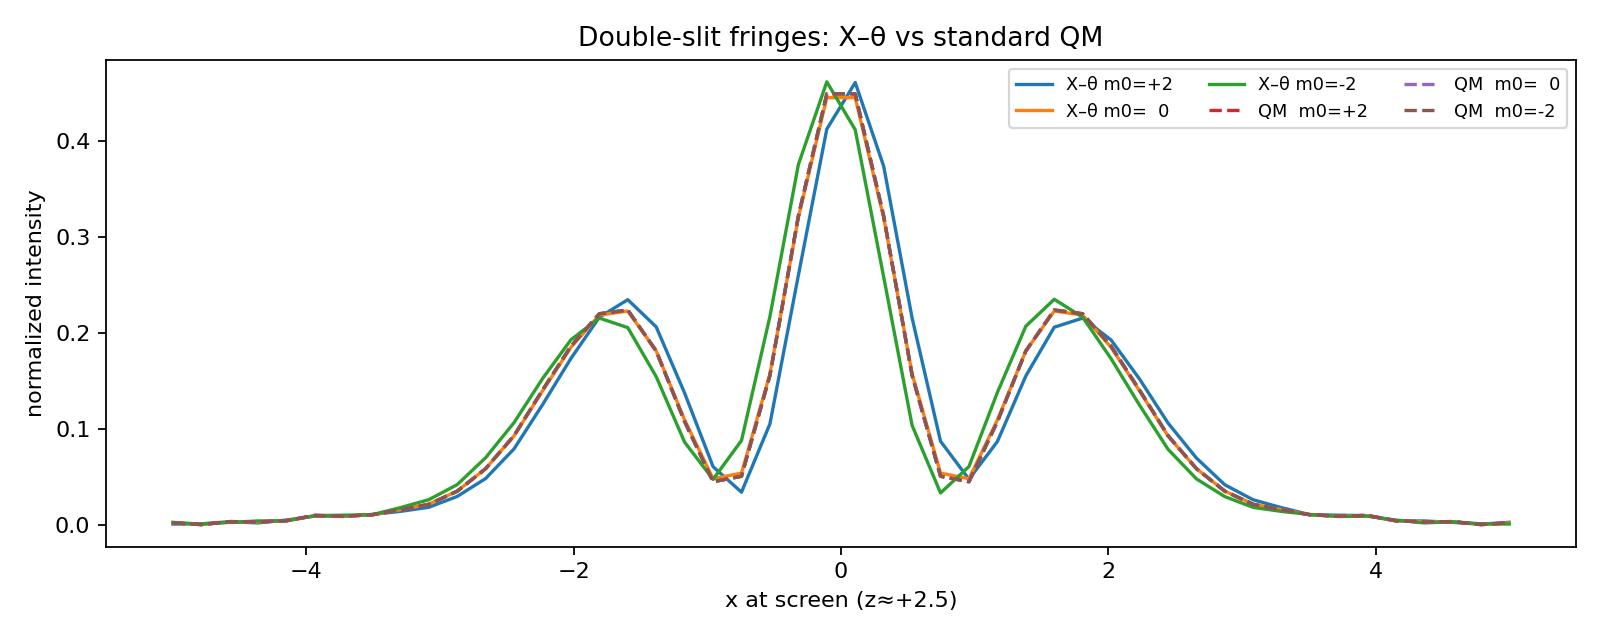
\includegraphics[width=0.85\linewidth]{neutron_atom_interferometry_theta.png}
  \caption{Simulated interferometry phase shifts with $\theta$ included.
  Tabletop experiments can test these signatures.}
  \label{fig:neutron-atom-interferometry}
\end{figure}
